%%%%%%%%%%%%%%%%%%%%%%%%%%%%%%%%%%%%%%%%%%%%%%%%%%%%%%%%%%%
% EPFL report package, main thesis file
% Goal: provide formatting for theses and project reports
% Author: Mathias Payer <mathias.payer@epfl.ch>
%
% This work may be distributed and/or modified under the
% conditions of the LaTeX Project Public License, either version 1.3
% of this license or (at your option) any later version.
% The latest version of this license is in
%   http://www.latex-project.org/lppl.txt
%
%%%%%%%%%%%%%%%%%%%%%%%%%%%%%%%%%%%%%%%%%%%%%%%%%%%%%%%%%%%
\documentclass[a4paper,11pt,oneside]{report}
% Options: MScThesis, BScThesis, MScProject, BScProject
\usepackage[BScProject,lablogo]{EPFLreport}
\usepackage{xspace}

\title{Multiple files support in Scastie,\\the interactive playground for Scala}
\author{David Kalajdzic}
\adviser{Professor Dr. Martin Odersky}
\supervisor{Jędrzej Rochala\\VirtusLab} %\\Software engineer at VirtusLab
\supervisorb{Julien Richard-Foy\\ScalaCenter}

\newcommand{\sysname}{FooSystem\xspace}


%%%%%%%%%%%%
\usepackage{listings}

\lstdefinestyle{sc}{
  frame=tb,
  language=scala,
  aboveskip=3mm,
  belowskip=3mm,
  showstringspaces=false,
  columns=flexible,
  basicstyle={\small\ttfamily},
  numbers=none,
  numberstyle=\tiny\color{gray},
  keywordstyle=\color{blue},
  commentstyle=\color{dkgreen},
  stringstyle=\color{mauve},
  frame=single,
  breaklines=true,
  breakatwhitespace=true,
  tabsize=3,
}

\lstset{style=sc}
%%%%%%%%%%%%

\begin{document}
\maketitle
% \makededication
% \makeacks

\begin{abstract}
Scastie is an online website that allows users to write and execute Scala code. It currently supports editing and running of only one code snippet. The goal of this project is to enhance Scastie to enable users to work with multiple files, facilitating better organization and management of complex projects.

This involves implementing a user interface for creating, opening, saving, and switching between files, as well as making backend modifications to handle multiple files effectively. The addition of multiple files support will improve the overall user experience and make Scastie a more versatile coding platform.
\end{abstract}

% \begin{frenchabstract}
% For a doctoral thesis, you have to provide a French translation of the
% English abstract. For other projects this is optional.
% \end{frenchabstract}

\maketoc

%%%%%%%%%%%%%%%%%%%%%%
\chapter{Introduction}
%%%%%%%%%%%%%%%%%%%%%%
\section{Presentation}
Scastie is an Open Source project maintained by the Scala Center lab, accessible at \href{https://scastie.scala-lang.org}{\color{blue}https://scastie.scala-lang.org}. It serves as an online website where users can store and execute code snippets. Its functionalities include sharing code snippets, switching between Scala versions, utilizing publicly available libraries, handling compilation errors, runtime errors, instrumentation, and more. Users can conveniently run Scala code remotely without the need for local setup.

\begin{figure}[h]
\centering
\includegraphics[width=8cm]{old.jpeg}
\caption{Original user interface}
\end{figure}

At this time the Scastie website only allows users to edit one code snippet (which represents one file). The snippet has two main modes of operation : normal mode (where the code is just a main.scala file) or worksheet mode which is similar to the .sc worksheet that some IDEs provide but with much more : we can interleave code and HTML blocks like Jupiter Notebooks.

Another functionality of the Scastie client is the Embedded mode of Scastie. Users can embedded the Scastie editor inside any website.

\section{Challenges}
Scastie, the online Scala playground, currently allows users to edit a single file at a time. However, this approach has limitations, particularly when dealing with larger, more complex snippets, or when macros are employed (to compile, macros need to be defined in a separate file).

My project aims to address these issues by introducing a new feature : multi-file editing. The envisioned user interface will mirror the dynamics of an IDE, with users able to create, rename, delete, and organize files within a hierarchical view.

It's important to note that worksheet mode will remain unaffected and continue to support single-file editing. However, upon disabling worksheet mode, users will gain the ability to write and organize multiple files within Scastie.

Specifically, I will:
\begin{enumerate}
\item Develop a UI for displaying multiple files (file hierarchy, tab switches).
\item Implement client-side logic for handling tab switches.
\item Implement server-side logic for compilation of multiple files
\item Still display compilation and runtime errors per file.
\item Enable auto-completion across files.
\item Ensure backward compatibility with existing features and snippets.
\end{enumerate}

The goal is to ensure that Scastie not only supports multi-file editing but also compiles multiple files properly on the server, maintains existing features, and provides basic IDE functionalities. 

In essence, this project is not merely an upgrade, it's a overhaul improvement of Scastie's usability, facilitating code organization, and supporting the use of macros. It's a challenging task, as it requires a deep understanding of Scastie's front-end and back-end. However, it promises to significantly improve the user experience and extend Scastie's capabilities.

%%%%%%%%%%%%%%%%%%%%
\chapter{Background}
%%%%%%%%%%%%%%%%%%%%

This section provides the necessary background to understand the changes that were made to support multiple files.

\begin{figure}[h]
\centering
\includegraphics[width=16.5cm]{ScastieArchitecture.png}
\caption{Scastie's architecture}
\end{figure}

Scastie's front end uses React, but it is written in Scala and powered by Scala.js and \href{https://github.com/japgolly/scalajs-react}{\color{blue}scalajs-react} library. Each Scastie front end communicates with the Scastie backend service using the HTTP protocol.
The server has an internal \lstinline{DispatchActor} that handles and redirects all user requests. In fact, the server distributes the load based on the sbt configuration chosen by the user for their code snippet and redirects it with the Akka protocol to a remote \lstinline{SbtRunner}. The \lstinline{SbtRunner} then launches the code in a local and independent sbt environment for specifically for that snippet.
This \lstinline{LoadBalancer} communicates with Futures to the storage component, allowing it to create/fork snippets in the database and store all the snippets that users have written.

Metals support was recently \href{https://github.com/scalacenter/scastie/pull/655}{\color{blue}{introduced}}, which includes basic features such as auto-completion and hover operations. It runs on a separate process from the server and is shared among all users.

%%%%%%%%%%%%%%%%
\chapter{Implementation}
%%%%%%%%%%%%%%%%
Here I will explain all changes I made, starting with front end and then with backend.

\section{Front end}

\subsection{Codebase}
Scastie's front end is developed using ScalaJS.React, which introduces complexity due to its non-standard syntax compared to JavaScript-based React. The lack of beginner-friendly documentation for the ScalaJS-React library made it necessary to first learn JavaScript-based React and then translate that knowledge to Scala.

Another challenge was that Scastie's client is undocumented and its entire code base had one \lstinline{Folder} with around 40 files. Those files were React components of very sparse abstraction levels (for instance we have the component \lstinline{NewButton} which allow users to create a new code snippet, sitting next to \lstinline{EmbeddedOverlay} component which is some overlay we display when the Scastie is in embedded mode). This introduces lot's of confusion. Especially because there is no documentation in the whole Scastie's front end, it gets difficult sometimes to understand what each component does and why.\\
My first job was to clean this code base so we organize files into logical folders so that we can navigate and understand the front end's code better. 

\subsection{\lstinline{ScastieState}}
All components composing the client will depend on one centralized UI state. Basically there is a \lstinline{ScastieState} case class that know everything about the view (which modal is showed, the code that user is writing, libraries, console state, boolean indicating if the line numbers are showed or not,...). Having one single source of truth is great because it avoid having duplicate information that we have to synchronise around the components, we have a main component that feeds down information to all components. But having all those fields that correspond to different abstraction levels is very confusing for the same reason as explained in the previous section.

During the project, my main objective was to incorporate multiple files support rather than refactoring the entire codebase. However, I made a conscious effort to avoid replicating the undesirable code style that existed previously.

Here I will explain changes I made :
\subsection{CSS}
Being able to insert a side file hierarchy view and tab strip view is going to be difficult because the CSS (Cascading Style Sheets) files heavily rely on the fact that there is one editor with just one console bellow it. Introducing multiple files is a great time to introduce proper responsive UI and refactor the whole CSS.

The initial UI was rudimentary and it described all component's dimensions with absolute values in the CSS. This worked for very simple UIs, but now that we want to start adding complexity and functionality in the UI, it it the right time to refactor the CSS (and it will avoid having something unmaintainable in the future).\\
To solve this I changed the layout by introducing some CSS grid layout and CSS Flexible Box Layout (flex layout) at the right places. They both allow to describe layouts and automatically compute dimensions of its elements, they can be equivalent but depending on the situation one might prefer to use one over the other. The main difference is that the grid allows to describe very strong structural layout whereas flex is much more flexible.


I used the box layout to define 3 big rows : one for the top bar (where I have inside a horizontal flex that has to the leading side the Scastie logo and the trailing few utils buttons such as the login one), a large central bar and the bottom bar with general infos (help, privacy policy, Scastie's Github link). See Figure \ref{grids}.

\begin{figure}[h]
\centering
\includegraphics[width=12cm]{main-grid.jpg}
\caption{CSS Box layout is used to enforce this structural view}
\label{grids}
\end{figure}

\newpage

This large central area is very flexible and will have a side-pane with the file hierarchy view and a central pane with the code editor as well as the tab bar on top and with the collapsable console in bottom.

Flex layout is appropriate because it allows to be very expressive in the behavior we want : need to change the direction of the file hierarchy and text editor views (on mobile the screen is not wide enough to have them side by side that's why for mobile it should display them in vertical direction as shown on the following figures \ref{iphone}.

\begin{figure}[h]
\centering
\includegraphics[height=7cm]{iphone.jpeg}
\includegraphics[height=7cm]{ipad.jpeg}
\caption{The file hierarchy view adapts for mobile and sits over the editor. Meanwhile for tablets it still remains on the side but with a reduced size compared to desktop}
\label{iphone}
\end{figure}

Moreover it simplifies a lot the CSS files, previously every components had hard-coded dimensions and the editor for instance was computing its size depending on the state and dimensions of elements nearby. For example the console when was opened it changed the CSS class of the editor so that forces it to recompute its size knowing that console's height has changed. Using flex layout allows to define how each elements shrink and behaves as dimensions are changing. As well as dynamically choosing what to show and hide while still allowing the components to take the maximum space they can. For example the file hierarchy view can be completely hidden or showed by clicking on the button, the same way VS-Code or IntelliJ IDEA do as Figure \ref{scrolls} shows.\\
This will make the client UI very easy to modify for any future functionalities. For example allowing the user to change the console or side pane's exact dimensions dynamically with the mouse.


\begin{figure}[h!]
\centering
\includegraphics[height=7cm]{scrollsA.jpeg}
\includegraphics[height=7cm]{scrolls.jpeg}
\caption{Text editor takes full space available, it shows scroll bars when it's content is too large. Toggling the side pane (which has a file hierarchy) and the console works as expected.}
\label{scrolls}
\end{figure}

\newpage

\subsection{File hierarchy}
The file hierarchy view is a visual representation of some data structure. It is interacting the model and then it gets refreshed thanks to the React technology. The UI will react to changes that occurred in the model, where those changes are initiated by users mouse. The file hierarchy view I made supports drag and drop of files and folders and insertion, deletion, renaming. 
When moving a \lstinline{Folder} it should not accept a drop in one of its recursive sub-folders. And moving a file should of course change its path, but when moving a \lstinline{Folder} it should change the \lstinline{Folder}'s path as well as all it's children (sub-folders and all files that are inside the \lstinline{Folder}).

I designed an folder hierarchy data structure that is in the form of a tree. Mainly a \lstinline{Folder} has children of type \lstinline{File} or \lstinline{Folder}. Each node (\lstinline{File} or \lstinline{Folder}) is a case class and has a path. The root folder starts with path $/$.\\
This data structure is immutable. And provides all basic operations that the view will need to use (move, insert, delete, find, ...)
A difficulty was that moving a \lstinline{Folder} is changing all its direct children path, and subsequent children of sub-folders, my solution is heavily based on pattern matching and recursive algorithm.

Opting for immutability was the appropriate choice in this scenario, especially when considering the usage of Scala.js React. The React mechanism relies on displaying the complete file hierarchy of a root \lstinline{Folder}. To ensure seamless integration with React, it is crucial not to provide direct mutation capabilities to the programmer. Modifying the displayed content with React involves complex operations that require using "modState()" and other React-specific techniques. By maintaining immutability in the data structure, we can simplify the interaction between the hierarchy and the React components.

The file hierarchy view component has a private case class \lstinline{FileHierarchyState} that describes the current component's state variables. Following the encapsulation paradigm we don't need to store this \lstinline{FileHierarchyState} in the global \lstinline{ScastieState} because it is just internal state that only the file hierarchy view needs (it has  information of which folders are expanded/collapsed and drag information).

\subsection{Tab strip}
\lstinline{TapStrip} has a \lstinline{TapStripState} case class but is handed by \lstinline{ScastieState}, because knowing which tab the user has opened is important information that is available in the central \lstinline{ScastieState}. Especially concerning compilation errors that must be filtered per file.

\subsection{Layer of components}
Quick note to explain how file hierarchy and tab strip communicate. When opening a file in the file hierarchy we need to create a tab in tab strip, as well as when we delete a file in file hierarchy we need to close it's tab. This logic is handled by a parent component which has those two components in it's view. To avoid complex communication across components, the more elegant design is that information that we share between two components is not duplicated, that there is one and only one source of truth. The parent component knows about its state and feed down to children as props. If the children want to change it, they call a \lstinline{Callback} that the parent will respond, that is mutate this shared state variables.


\subsection{Extras}
I did some extra work:
\begin{itemize}
    \item Introduced a thin side bar so the UI looks more like an IDE and allows fast switching between file hierarchy and  build settings views.
    \item Build settings goes inside the big side-pane which and thus replaces the file hierarchy view
    \item Embed mode allows users to publish Scastie snippets inside external websites. Some websites heavily rely on that feature \footnote{\url{https://tourofscala.com/}} \footnote{\url{https://virtuslab.github.io/scala-yaml/docs/index.html}}. We want to display the file hierarchy if and only if there is more than one file in the source code. This is very easy to do thanks to how I structured the UI. Just hiding the elements we don't want is enough, all others will take that available space dynamically.
    \item Presentation mode hides tab strip and increases font size while still being able to navigation across files with file hierarchy.
\end{itemize}

\begin{figure}[h]
\centering
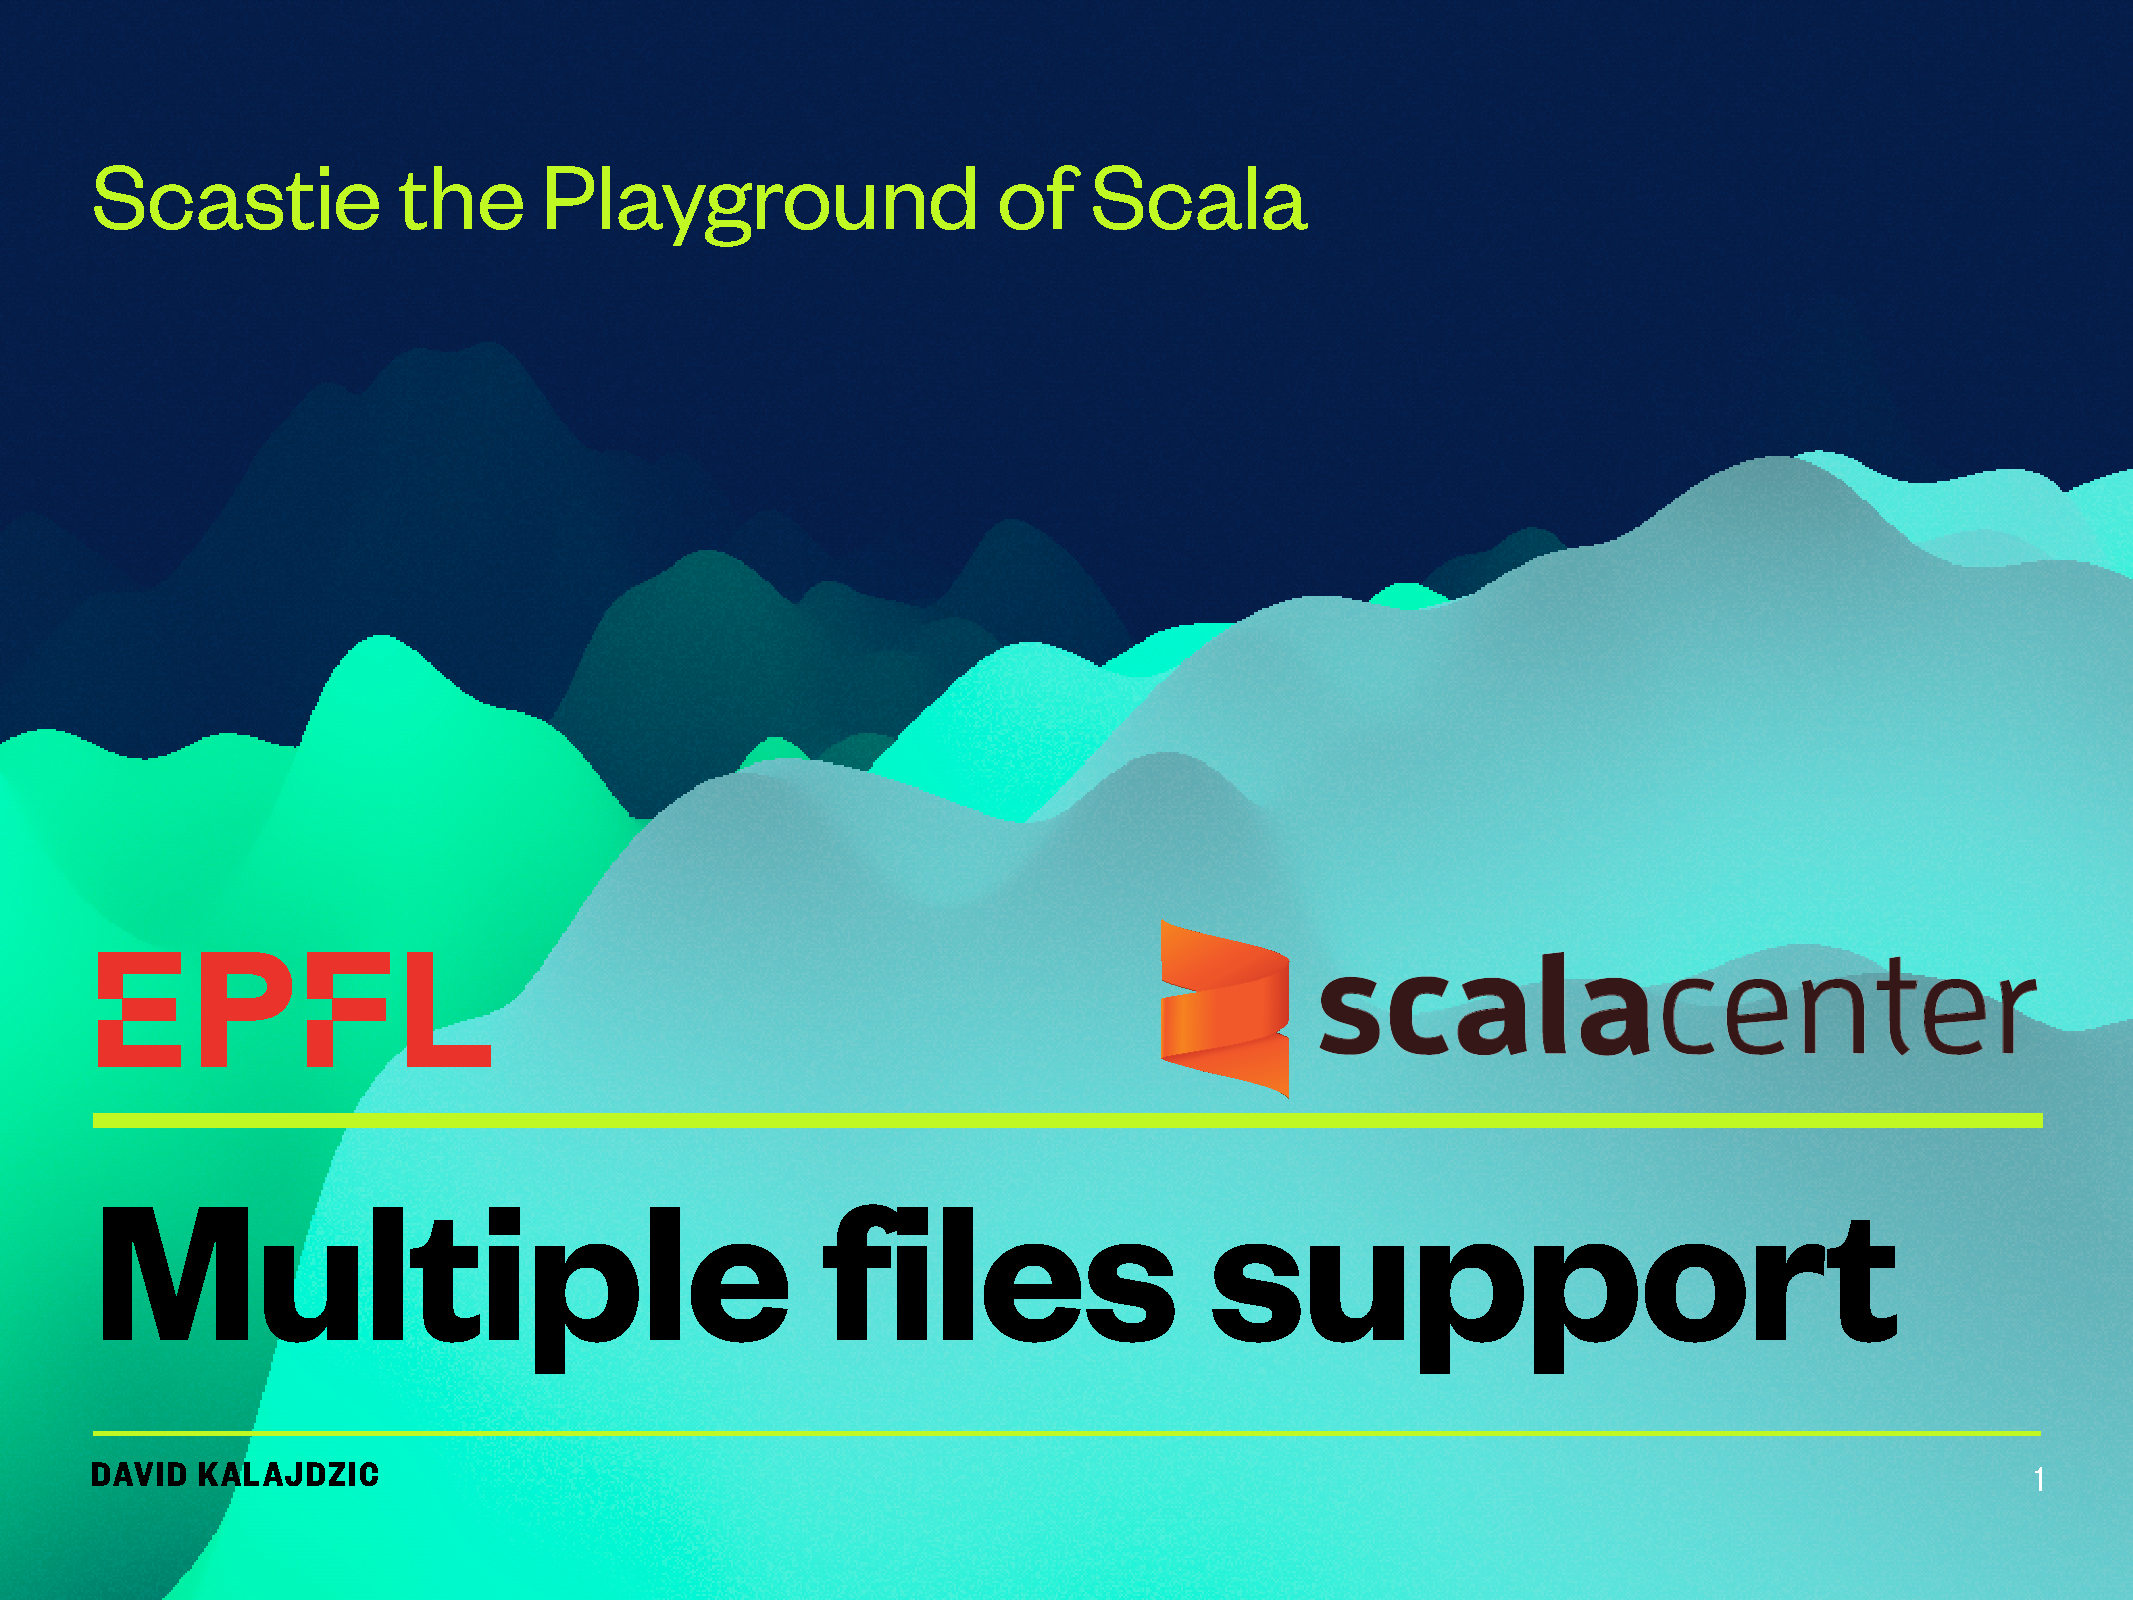
\includegraphics[height=7cm]{presentation.jpeg}
\caption{The presentation mode with multiple files editing}
\label{presentation}
\end{figure}

\newpage
\section{Back end}
% backward compatibility
% inputs code string -> \lstinline{Folder}
% sbt process multiple files
% per file compilation and runtime infos
% migration script compatible for future migrations
% code formatting
% metas0s presentation compiler
% currently no valid api solutoin for this ther eis no method in presetnaioncompiler
% tests that prove that i did is working
% zip

The Scastie backend is very complex, it has a huge technical dept because it mixes and uses a lot of different technologies, such as Akka. The code is rather difficult to understand because Akka actors are everywhere and no documentation exists.

\subsection{Backward compatibility\label{backcomp}}
This is the main constraint in this project. We want that existing code snippets still remain compatible with this multiple files support. That is that old snippets can be turned into multiple files snippets. At present, millions of code snippets, encapsulated as \lstinline{MongoSnippet} case classes, are stored in a MongoDB database.

A \lstinline{MongoSnippet} contains an Inputs case class field. This field regroups various properties, including the Scala version, libraries, worksheet mode, and a crucial 'code' property, which is a String. This string represents the source code of the snippet. I have developed a file hierarchy data structure, referred to as a \lstinline{Folder} tree. Our ideal objective is to substitute the 'code' property's String type with this \lstinline{Folder} type.

This change cannot be backward compatible (and then couldn't exploit the flexibility of NoSQL databases). In fact we either need to migrate all the current database to the new format at once. Or we migrate each item on the fly as old snippets will be fetched from users.

Following a detailed discussion with the project supervisor, we decided that conducting a full-scale migration was a more viable and cleaner approach. In the future, we'll always need to use multiple files, so it's important to change the model and the database to this new format. Creating code that changes the data on the fly is often what is done in large-scale application to avoid this expensive task of database migrations, but this would make our code more complicated. This could also slow things down and make the code harder to read and maintain because we'd have to be very careful with it.

\subsection{Migration script}
Migration of the database from the previous \lstinline{MongoSnippet}, which had a string for its code, to the \lstinline{Folder} structure, was done through a standalone migration program. This involves defining \lstinline{MongoSnippetV1} and \lstinline{MongoSnippetV2} case classes, along with a function to translate from V1 to V2. This generalized approach ensures the program can be reused for any future migration scripts that might be needed.

I opted to not mutate each snippet in the Mongo Collection one by one, but to follow more like a functional programming approach. The idea is that the migration takes as input a collection of snippet with type \lstinline{MongoSnippetV1} and it will be migrated into a newly created collection (with type \lstinline{MongoSnippetV2}). This allows this migration script to not be destructive and thus can rerun the script as many times as needed (it will create each time a new collection).

This method also facilitates checks for script correctness by comparing the original and transformed collections.

The script works as follows : 
\begin{enumerate}
\item We fetch all snippet ids from the 'snippets' collection.
\item For each snippet ID, retrieve the corresponding \lstinline{MongoSnippet}, modify it, and store it in the new collection. We create a \lstinline{Folder} hierarchy that contains a single main.scala file, the content of which is the String code from the respective \lstinline{MongoSnippetV1}.
\item We finally add the same MongoDB indexes to that new collection.
\end{enumerate}

The script starts by retrieving all snippet IDs from the 'snippets' collection. I opted for this method to avoid potential memory overflow that could occur if we tried to fetch all \lstinline{MongoSnippet}s at once, especially when dealing with large collections. By fetching only the IDs first, we keep the memory usage to a minimum.

Finally upon successful completion of the migration script, the person in charge of production can simply rename this new collection and delete the old one, if it's no longer needed.

\subsection{Inputs}
As mentioned in \ref{backcomp}, I have made a modification to the input parameter 'code' String, replacing it with '\lstinline{Folder}'. This change has significant implications for numerous files, necessitating a thorough comprehension of their usage and the underlying principles of Scastie. Understanding these aspects is vital to successfully implementing support for multiple files. The following are essential areas that required modifications to accommodate this feature:

\subsection{\lstinline{SbtProcess}}
When the user wants to run a snippet it will make a http request to the main server which will redirect that query to the \lstinline{LoadBalancer}. This balancer will select the best \lstinline{SbtRunner} available to run the snippet. (the most suitable \lstinline{SbtRunner} is determined based on its compatibility with the snippet's Inputs libraries configuration, Scala version, availability, among other factors.)

Finally the \lstinline{SbtRunner}'s \lstinline{SbtActor} will forward the task to \lstinline{SbtProcess}. \lstinline{SbtProcess} is a \lstinline{ProcessActor} that interacts in command line with a sbt instance.
It writes a little sbt project in some \lstinline{sbtDirectory} on file system, then it programmatically compiles it (by making $reload;compile/compileInputs$) and then makes a \lstinline{sbtRunCommand} (which depends on the Scala Target, but basically a $fgRun$)

The \lstinline{SbtProcess} needs now to not simply overwrite some main.scala file in this sbt working directory but to replace them by the \lstinline{Folder} hierarchy files. Because the \lstinline{SbtProcess} can be reused across users (load balancer decides) it is important to delete all files before writing the new ones on disk and compile and run those new ones to avoid any conflicts.

\subsection{Compilation \& Runtime infos}
Currently in Scastie both compile-time and runtime errors are displayed to the user. They appear as a red dot in the exact line number with the error message. It is important to keep this feature for the multiple files functionality. In fact we need to retrieved and propagate and finally display the correct error message for the specific file.

There is a custom made sbt plugin which is called \lstinline{sbt-scastie}. It is a plugin that allows to report both errors and console output and will be injected to all \lstinline{SbtRunner}s.
This plugin is printing information in JSON format to standard console, which on the receiver end (the \lstinline{OutputExtractor} object in Scastie's \lstinline{SbtRunner}) will be parsed back into the original case class format.

This \lstinline{sbt-scastie} plugin embarks a custom compiler reporter which captures all warning and compilation problems. These issues are encapsulated in a \lstinline{Problem} case class which is then printed to the standard output in a JSON format by that plugin.\\
Similarly this plugin has a mechanism to handle runtime errors, capturing all runtime output, including error messages. These messages are formatted into \lstinline{ConsoleOutput} or \lstinline{RuntimeErrorWrap} case classes, representing regular console output or runtime error messages, respectively. These case classes are also converted into a JSON format and printed to the standard output.

To support multiple files, it is necessary to include the source file path of each error. To achieve this, I enhanced the \lstinline{Problem} and \lstinline{RuntimeErrorWrap} case classes by extracting the file path from the position information provided by \lstinline{xsbti.Problem}. By adding a new field to these classes, the file path where the error originated is recorded. 

Scastie now offers its users exact and helpful feedback on their multi-file code by capturing the file-specific origin of each issue and accurately correlating it with its associated file. This strategy promotes effective debugging and enhances the user experience.

\subsection{Metals support}
Metals is a powerful language server for Scala. It provides all the rich editing features expected in modern IDEs, such as code completion, hints, navigation, and finding references.

In Scastie, Metals is running on a separate and independent process. Currently for each Scala target version, a separate, cached \lstinline{PresentationCompiler} is assigned.\\
The \lstinline{PresentationCompiler} is a part of the Scala Compiler designed to support IDE functionalities like type inference, auto-completion, and hyperlinking to definitions. It operates incrementally, constantly updating its understanding of the code as it is edited to provide real-time, contextual insights and assistance.

On the Scastie frontend, whenever a user hovers the mouse over a parameter, types code, or invokes the auto-complete function (Ctrl+space), a request is sent to Scastie's Metals. This request includes the current text editor's content and cursor location, enabling the \lstinline{PresentationCompiler} to adapt its response based on the ongoing edits.

During my project, I discovered that a \lstinline{ScastiePresentationCompiler} is shared among multiple users (in fact among those using non-worksheet mode with the same Scala Target and dependencies), leading to potential information leaks. This vulnerability, which could result in one user receiving code completion hints intended for another user will need addressing in the future.

A particular issue is that auto-completion currently fails if the method to be auto-completed is located in another file. Unfortunately the \lstinline{PresentationCompiler} does not support multiple files editing, currently there is no valid method to provide all files to this presentation to be able to complete from another file.

The way that Metals is integrated into Scastie needs significant improvements. It should go beyond the basic implementation of the \lstinline{PresentationCompiler} and be thoroughly reworked.

My solution in the meantime is to create a $/setup$ web API endpoint which will be called when the users open a snippet in their browser. This setup will provide all the Scala files the user will be editing and then this \lstinline{PresentationCompiler} will track the source code's evolution as the user types in the code editor. \\
At its core, the $/setup$ function performs a $/complete$ operation on each file's content. This approach allows me to exploit a bug in Metals where a shared \lstinline{PresentationCompiler} inadvertently provides access to code completions from other files.

Finally all this ensures that auto-completion works across multiple files in a project. While this isn't a perfect solution, it avoids the need for a complete rewrite of the Metals integration in Scastie, which isn't within the scope of this project.

\begin{figure}[h]
\centering
\includegraphics[height=9cm]{completion.jpeg}
\caption{Auto-completion and hover are working in this multiple files project}
\end{figure}

\subsection{Extras}

With careful consideration for detail, I've also ensured that both code formatting and project zip download buttons still work as expected.\\
Code formatting depends on the currently selected file and therefore must propagate until the FormatActor only the currently selected file's content.\\
Exporting a multiple-file snippet as a Zip archive is still supported (it is necessary to export all files, maintaining the \lstinline{Folder} hierarchy).

Finally, with all these modifications, the addition of the multi-file feature for Scastie has not disrupted any existing functionality.

%%%%%%%%%%%%%%%%%%%%
\chapter{Evaluation}
%%%%%%%%%%%%%%%%%%%%
The project goal is to extend Scastie by allowing users to edit multiple files instead of one big file. This will enable better organization, understanding, and navigation in the source code.

Multiple files support should not only be handled in the frontend (a simple hack would have been to edit a large code file by splitting its content into different view editors but merging them altogether in one giant file; this would be a frontend-only solution), but deeply integrated into the Scastie website. It should actually generate and compile multiple files. This will now allow users to write Macros in Scastie.

Macros cannot be defined in the same Scala file where they are used. Running a Scastie snippet using macros is a sufficient way to prove that there is indeed real multiple file support.

To evaluate the correctness of my project, I wrote tests in the backend. The \lstinline{SbtRunner} is being tested by running not only a one-file Scastie program but also a whole folder hierarchy. The tests will check the correctness of accessing a def from another file, as well as the Macros functionality.

There is also a test to check that compilation and runtime errors provide the correct file name location of the error.

Regarding Metals, I wrote tests that check if auto-completion works across files.

Finally, concerning the UI, it was tested manually. Performance and responsiveness across different screen sizes and browser versions have been checked manually.

%%%%%%%%%%%%%%%%%%%%
\chapter{Conclusion}
%%%%%%%%%%%%%%%%%%%%

The goal of the project was to extend Scastie, an online Scala editor, to support the editing of multiple files. This feature would enable users to organize, understand, and navigate source code more effectively, and support macro definitions. The extension was not merely to be implemented at the frontend, but at a deeper level within Scastie itself.

The assignment was challenging and called requiring a thorough understanding of Scastie's architecture and the numerous technologies it uses, including Akka and Metals, a Scala language server. 
There were additional levels of complexity due to the system's significant technological debt and the lack of any kind of documentation. The codebase was challenging to comprehend and navigate.

A key constraint was maintaining backward compatibility, ensuring that existing code snippets remained functional with the new multi-file support as well as all functionalities.

Although this was my first time dealing with such a real world project, the experience provided invaluable insights into working in a large Scala codebase, data migration, backward compatibility, and other real-world concerns. It underscored the importance of clear communication across various components of an application, the necessity of maintaining a single source of truth, and the potential complexities that can arise in large-scale applications.

This project has significantly extended the capabilities of Scastie, and while there are areas that need further improvement, such as the Metals, the achievement of real multi-file support in Scastie is a considerable accomplishment. It will not only benefit users in terms of code organization and navigation, but also allow them to work with macros, which was previously impossible.

\cleardoublepage
\phantomsection
\addcontentsline{toc}{chapter}{Bibliography}
\printbibliography

% Appendices are optional
% \appendix
% %%%%%%%%%%%%%%%%%%%%%%%%%%%%%%%%%%%%%%
% \chapter{How to make a transmogrifier}
% %%%%%%%%%%%%%%%%%%%%%%%%%%%%%%%%%%%%%%
%
% In case you ever need an (optional) appendix.
%
% You need the following items:
% \begin{itemize}
% \item A box
% \item Crayons
% \item A self-aware 5-year old
% \end{itemize}

\end{document}